\documentclass{article}
\usepackage[utf8]{inputenc}
\usepackage[T1]{fontenc}

\usepackage{tikz} % used for drawing
\usepackage{listings} % used for programming code
\usepackage{float}
\usepackage[a4paper]{geometry}

\lstset{frame=leftline}

\lstdefinelanguage{Gherkin}{
  keywords={When, Then, Given, And},
  ndkeywords={Feature, Scenario},
  sensitive=false,
  comment=[l]{\#},
  morestring=[b]',
  morestring=[b]"
}

\title{Splay : Basics}
\author{Rémy Voet \& Samuel Monroe}

\date{\today}

\geometry{hscale=0.70,vscale=0.85,centering}

\begin{document}
\maketitle

\section{Introduction}

  This document contains our first thoughts on the future of the Splay project
  and the direction we would like to take for our thesis.\\

  We'll first approach the architecture modifications we would like to
  make, and why these would make sense within the project.\\
  This will be followed by our first \textbf{User Scenarios}, how we
  would like the application to be used and thus giving us precise goal and
  specifications for further work.\\

  This document will end with a section about some thoughts about the
  application not directly concerning the user scenarios goals but
  worthing, in our opinion, to be discussed.

\section{Architecture Modifications}

  This is the current architecture of Splay as it is today : \\

  \begin{figure}[H]
   \caption{\label{curr_arch} Current Splay Architecture}
   \centering
   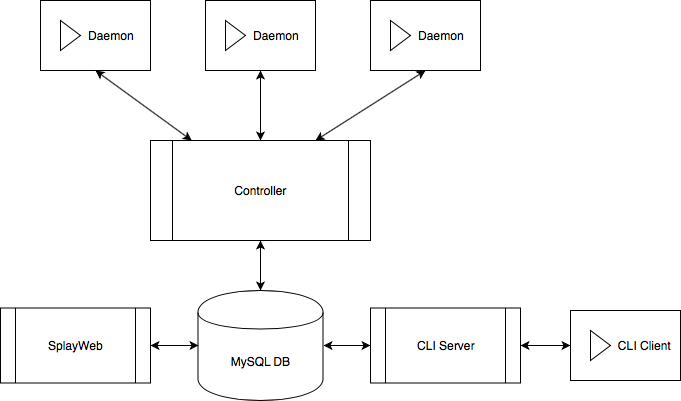
\includegraphics[scale=0.6]{images/curr_arch.png}
  \end{figure}

  During our part-time job on upgrading Splay version, we found out
  that \textbf{CLI Server} and \textbf{SplayWeb} (into backend) were a huge place
  of code duplication. Indeed, they provide the same kind of interactions
  with the DB, except one is in a web interface and the other is in a
  command-line interface.\\

  We would therefore like to change the architecture for this one : \\

  \begin{figure}[H]
   \caption{\label{new_arch} Desired Splay Architecture}
   \centering
   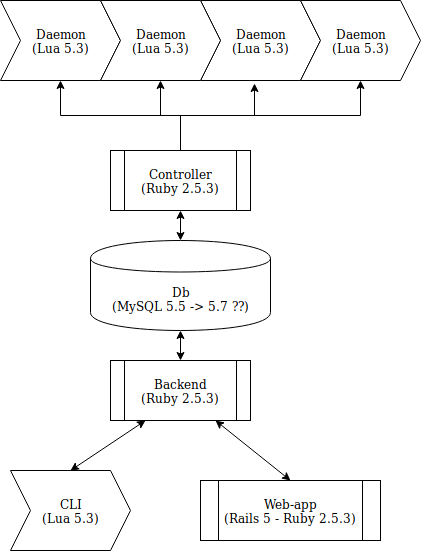
\includegraphics[scale=0.6]{images/NewSplay.png}
  \end{figure}

  The interactions with the DB would then be unified and would make
  lighter clients both for the web and CLI part, just making use of
  the available JSON API.\\

  Basically, that refactor would be easy to implement as it would be the
  matter of setting up the now-called \textbf{CLI Server} as our
  controller with the JSON API, then slightly refactoring the CLI client
  and building a lightweight web app around it (it may also be a refactoring
  of the current Rails app).\\

\section{User Scenarios}

  The main use scenario we want to focus on is the student usage
  through the raspberry cluster, allowing him to test his distributed
  algorithm and browse statistics about the nodes and the algorithm result.\\

    \begin{lstlisting}[language=Gherkin]
    Feature: As student
             In order to test my distributed algorithm
             I want to submit it to the application and receive stats about it

      Scenario: A registered student submit his algorithm through the web-app
        Given I am registered and logged in
        When I go on the algorithm submission page
        And I paste my algorithm
        And I submit the form
        Then I am prompted with a confirmation
        When the algorithm is done
        Then I can see stats about the algorithm execution on the nodes
    \end{lstlisting}

    \begin{lstlisting}[language=Gherkin]
    Feature: As student
             In order to test my distributed algorithm resilience
             I want to be able to configure failure parameters for the execution

      Scenario: A registered student submit his algorithm through the web-app
        Given I am registered and logged in
        When I go on the algorithm submission page
        And I paste my algorithm
        And I select failure option on nodes or the network
        And I submit the form
        Then I am prompted with a confirmation
        When the execution is done
        Then I can see the result and statistics of it
        And I can see how the failure parameters influenced the execution
  \end{lstlisting}


\section{Thoughts and Ideas on Splay - Further Evolutions}

  \subsection{Testing}

    This is, for us, a mandatory change that must be introduced in the project.\\

    Currently, there are only few tests available for the Splay project,
    and they're not really usable or useful.\\
    We therefore would like to introduce two types of testing : \\
    \begin{itemize}
      \item Unit testing for particular parts of the code, and in
      every project's parts.
      \item Behaviour Driven Development testing. Creating test reproducing
      user interaction with the application would greatly ease the development
      by creating precise scenarios with Gherkin notation, and would help
      to test the application in a broader way.
    \end{itemize}

    Moreover, having a solid test-suite would make us more confident for
    pursuing new changes and improvements, but also making the application
    more maintainable in the future.



  \subsection{DB as the communication center}

    Currently, the MySQL (v5.5) database is the centralized and unique way for
    a user to interact with the Controller and Daemons.\\

    Our major concerns about this are : \\
    \begin{itemize}
      \item That DB is a potential bottleneck in the view of scaling the
      application for a web and wide usage, with a lot of Controller being
      created by user and relying on the DB to accomplish their job.
      \item The controller are constantly polling and
      querying that DB, and interact between themselves, assign jobs, basically
      do everything. Once again, this might be totally suitable for local usage,
      but scaling options are very limited.
    \end{itemize}

    As said before, this way of doing things will be perfect for a low-scaled
    usage on a raspberry cluster, which is in the end one of the main goal
    of our thesis.\\
    But options like Redis \cite{redispubsub} for replacing the communication channel with a
    Publish/Subscribe service might be somehow an idea of improvement.

  \subsection{Rewriting part of the application}

    As said during the first meeting, rewriting parts of the application
    is certainly not a priority for this thesis, as we might get caught up in
    some infernal trap of being unable to rewrite in reasonable times.\\

    But we do still believe that a functional language like Elixir \cite{elixir}, which
    is based on Erlang \cite{erlang}, might be more than suitable for this project.\\
    Indeed, the language doesn't solve the whole problem, but being able to
    work with a functional language, built to scale up and blow away concurrency
    problems, and providing the awesome OTP library \cite{otp}.\\

    Indeed we can sum up our needs by the following : \\
    \begin{itemize}
      \item We want a centralized way for the user to push jobs to some service
      knowing which machines it has access to (in this case, the raspberries).
      \item The service (controller) should be able to send the jobs to the workers,
      monitor what's going on on each worker, and have realtime feedback on the
      running jobs and the worker state.
      \item The worker should be able to talk to each other to accomplish the
      given job.
      \item We want the system to be resilient, but also to have complete
      control on the way jobs are accomplish (for instance, to make them
      crash on one worker and see that the \textit{leader election} algorithm
      is still accomplished by valid nodes).
      \item We want the cluster to be resilient, a crashed node should not stay crashed
      and force the user to restart the whole thing.
    \end{itemize}

    Elixir's OTP would be a way to achieve this and provide real scaling advantages
    if the system was to be put on the Cloud for wide access.\\
    A registered user could just log in the application, and ask for a job to be
    done. The system would spawn erlang processes dedicated to that task without
    even slowing down the other's experience.\\

    On the local cluster, the distributed system could be supervised by
    OTP's Supervisor \cite{elixirsupervisor} functionality, so that it never
    totally crash.\\


\nocite{*}
\bibliographystyle{plain}
\bibliography{bibli}

\end{document}
